%!TEX program=xelatex
\documentclass[UTF-8, a4paper, 12pt]{ctexart}
\setlength{\parindent}{0pt}
\usepackage{setspace}
\renewcommand{\baselinestretch}{1.5}
\usepackage{tikz}
\usepackage{pgfplots}
\usepackage{textcomp}
\usepackage[left=2.50cm, right=2.50cm, top=2.50cm, bottom=2.50cm]{geometry}
\usepackage{fancyhdr}
\usepackage{enumerate}
\pagestyle{fancy}
\rhead{\center{\small{华南理工大学大学城校区物理实验报告}}}

\begin{document}
    \begin{center}
        \zihao{-2}\heiti{分光计的调整与使用 预习报告}

        \zihao{-4}\songti{2020级 \quad 计算机科学与技术(全英创新班)\quad 王樾}
    \end{center}
    \zihao{4}\heiti{引言:}\zihao{-4}
    \songti
    分光计是精确测量光线偏转角的经典光学仪器。分光仪可借助棱镜将一束混合光分成不同角度的多束纯光,可用于折射率、光波长的测量与光谱分析。学习如何使用分光计能为今后使用更为精密的光学仪器打下良好基础。

    \textbf{\zihao{4} \heiti{一、实验目的}}

    \zihao{-4}\songti

    \begin{enumerate}[(1)]
        \item 了解分光计的构造、作用与工作原理。
        \item 掌握分光计的调整和使用方法。
        \item 用分光计测棱镜的折射率。
    \end{enumerate}

    \textbf{\zihao{4} \heiti{二、实验仪器}}

    \zihao{-4}\songti

    分光计、三棱镜、反射镜、汞灯。

    \textbf{\zihao{4} \heiti{三、实验原理}}

    \zihao{-4}\songti

    测量光线之间的夹角,其实等价于测量平行光束的方位角。当平行光管正确调整完毕后,焦平面上的每一个点都与一个方向上的平行光束相对应,而光轴在此之间转过的角度即是对应平行光束之间的夹角。

    我们使用最小偏向角法进行测量三棱镜折射率$n$,即当入射角等于出射角时,出现最小偏向角$\theta_0$,设棱镜顶角为$\varphi$,则折射率可表达为
    
    $$n = \frac{\sin \frac{\theta_0 + \varphi}{2}}{\sin \frac \varphi 2}$$

    证明如下:

    \begin{center}
        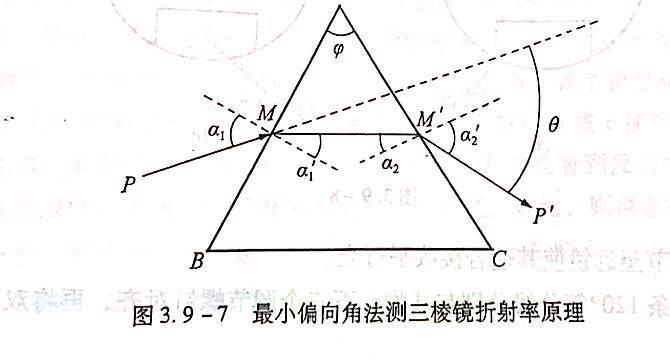
\includegraphics[width=0.80\textwidth]{proof_3.9.jpg}
    \end{center}

    由折射率定义(司乃尔定律),可得

    $$n = \frac{\sin \alpha_1}{\sin \alpha_1'} = \frac{\sin \alpha_2}{\sin \alpha_2'}$$

    由几何关系得:

    $$\alpha_1' + \alpha_2 = \varphi$$

    $$\theta = (\alpha_1 - \alpha_1') + (\alpha_2' - \alpha_2) = \alpha_1 + \alpha_2' - \varphi$$

    要求最小偏向角,可令$\frac{d\theta}{d\alpha_1} = 0$,此时有$0 = 1 + \frac{d\alpha_2'}{d\alpha_1} - 0$,即$$d\alpha_2' = -d\alpha_1$$

    对$\alpha_1' + \alpha_2 = \varphi$求微分,有$d\alpha_1' + d\alpha_2 = 0$,即$$d\alpha_2 = -d\alpha_1'$$

    对$\sin \alpha_1 = n \sin \alpha_1'$求微分,有$\cos \alpha_1 d\alpha_1 = n \cos \alpha_1' d\alpha_1'$

    有$\sin \alpha_2 = n \sin \alpha_2'$求微分,有$\cos \alpha_2 d \alpha_2 = n \cos \alpha_2' d\alpha_2'$

    若$\frac{d\theta}{d\alpha_1} = 0$,则有

    $$\frac{d\alpha_2}{d\alpha_1} = \frac{\cos \alpha_2' d\alpha_2'}{n\cos \alpha_2 d\alpha_1} = -\frac{\cos \alpha_2'}{n\cos \alpha_2}$$

    而固有

    $$\frac{d\alpha_2}{d\alpha_1} = \frac{-d\alpha_1'}{d\alpha_1} = -\frac{\cos \alpha_1 d\alpha_1}{n\cos \alpha_1' d\alpha_1} = -\frac{\cos \alpha_1}{n\cos \alpha_1'}$$
    
    联立两式,得$$\cos \alpha_1 \cos \alpha_2 = \cos \alpha_1' \cos \alpha_2'$$

    由对称性可知,当且仅当$\alpha_1 = \alpha_2', \alpha_1' = \alpha_2$时,上式成立,即$\frac{d\theta}{d\alpha_1} = 0$。

    记最小偏向角为$\theta_0$,则此时有$$\alpha_1' = \alpha_2 = \frac{\varphi}{2},\quad  \alpha_1 = \alpha_2' = \frac{\theta_0 + \varphi}{2}$$

    故偏向角公式为$$n = \frac{\sin \alpha_1}{\sin \alpha_1'} = \frac{\sin \frac{\theta_0 + \varphi}{2}}{\sin \frac{\varphi}{2}}$$

    \textbf{\zihao{4} \heiti{四、内容步骤}}

    \zihao{-4}\songti

    \begin{enumerate}[(1)]
        \item 调节分光计。调节分光计需要先目测粗调后进行细调,细调时在需要使用各半调节法将亮“十”字调到准线上方交叉点。
        \item 测量最小偏向角。将三棱镜置于载物台,旋转望远镜,寻找狭缝像。此后沿着偏向角减小的方向旋转,当随着游标盘转动而移动的狭缝像正要开始 反方向移动时,即为相应的折射光线最小偏向角的位置。
        \item 测三棱镜的顶角。将望远镜对准三棱镜的AB面,按自准直法调节,找到AB面反射得到的亮“十”字,记录左右游标读数$\alpha_3, \alpha_3'$,再将望远镜对准AC面,进行相似操作,记录左右游标读数$\alpha_4, \alpha_4'$。最终可得$$\varphi = 180^\circ - \frac{|\alpha_3 - \alpha_4| + |\alpha_3' - \alpha_4'|}{2}$$
    \end{enumerate}

\end{document}